\newpage
\section{Sequences \& Series}

\subsection{Definitions and notation}
\label{sec:6-1}
% CN 6.1

\begin{definition}[Sequence]
A \emph{sequence} is a function whose domain is $\N$ (an \emph{infinite sequence}) or $\{1,\dots,n\}$ for some $n$ (a \emph{finite sequence}, i.e.\ an ordered $n$-tuple, \S\ref{sec:1-14}).
\end{definition}

\begin{definition}[Term, length]
For a sequence $f$, the value $f(n)$, also written $f_n$, is its \emph{$n$-th term}. The \emph{length} of a finite sequence is the number of its terms, i.e.\ the size of its domain.
\end{definition}

\begin{note}[Indexing from $0$]
Some books index sequences from $0$ instead of $1$, i.e.\ use domain $\{0,1,2,\dots\}$. This only shifts the subscripts; the sequence is the same.
\end{note}

\begin{note}[Ways to specify a sequence]
\begin{itemize}
    \item List all its terms (only practical if it is short).
    \item Give a formula for the $n$-th term, e.g.\ $(n^2 : n\in\N)$ or $(n^2)_{n=1}^{\infty}$. This is like set-builder notation (\S\ref{sec:1-2}), but with parentheses because order matters.
    \item Give a recurrence relation (\S\ref{sec:6-2}), defining each term from earlier ones.
\end{itemize}
Listing a few terms and trusting the ``pattern'' does \emph{not} define a sequence: infinitely many different sequences start the same way. For example, $1,2,4,8,16$ continues as $32$ if $f_n=2^{n-1}$, but as $31$ if $f_n$ is the number of regions formed by joining $n$ points on a circle.
\end{note}

\subsection{Recursive definitions of sequences}
\label{sec:6-2}
% CN 6.2

\begin{definition}[Recurrence relation]
A \emph{recurrence relation} for $(a_n)$ expresses $a_n$ in terms of one or more earlier terms, together with enough \emph{base cases} (initial terms given explicitly) to determine every term uniquely.
\end{definition}

\begin{note}[Same shape as induction]
A recursive definition has a \textbf{base case}, defining finitely many of the simplest terms directly, and a \textbf{recursive case}, defining a general term from earlier ones. This mirrors the base case and inductive step of a proof by induction, which is why induction is the natural way to prove things about recursively defined sequences.
\end{note}

\begin{example}
\begin{itemize}
    \item $f_1=1$, $f_n=f_{n-1}+2$ gives $1,3,5,7,\dots$ (the odd numbers).
    \item $f_1=0$, $f_n=f_{n-1}+2$ gives $0,2,4,6,\dots$: the same rule with a different base case gives a different sequence.
    \item $f_1=1$, $f_n=nf_{n-1}$ gives $1,2,6,24,120,\dots$, i.e.\ $f_n=n!$.
\end{itemize}
\end{example}

\begin{note}[Multiple base cases]
A rule such as $f_n=4f_{n-2}$, which looks \emph{two} terms back, needs two base cases $f_1,f_2$; one base case alone fixes only every other term. For example, $f_1=2$, $f_2=0$, $f_n=4f_{n-2}$ gives $2,0,8,0,32,0,\dots$
\end{note}

\subsection{Arithmetic sequences}
\label{sec:6-3}
% CN 6.3

\begin{definition}[Arithmetic sequence]
An \emph{arithmetic sequence} has a constant difference $d$ between consecutive terms: $f_1=a$, $f_n=f_{n-1}+d$. Its $n$-th term is $a+(n-1)d$.
\end{definition}

\begin{example}
The positive integers ($a=1,d=1$), the odd numbers ($a=1,d=2$), and $10,7,4,1,-2,\dots$ ($a=10,d=-3$).
\end{example}

\subsection{Geometric sequences}
\label{sec:6-4}
% CN 6.4

\begin{definition}[Geometric sequence]
A \emph{geometric sequence} has a constant ratio $r$ between consecutive terms: $f_1=a$, $f_n=f_{n-1}\cdot r$. Its $n$-th term is $ar^{n-1}$.
\end{definition}

\begin{example}
The powers of $2$, $1,2,4,8,\dots$ ($a=1,r=2$), and $1,\frac12,\frac14,\frac18,\dots$ ($a=1,r=\frac12$).
\end{example}

\begin{note}[Arithmetic vs.\ geometric]
Arithmetic sequences grow by \emph{adding} the same amount each time; geometric sequences grow by \emph{multiplying} by the same amount. For $r>1$, geometric growth eventually beats any arithmetic growth.
\end{note}

\subsection{Harmonic sequences}
\label{sec:6-5}
% CN 6.5

\begin{definition}[Harmonic sequence]
$(a_n)$ is \emph{harmonic} if $(1/a_n)$ is arithmetic.
\end{definition}

\begin{example}
$(1/n : n\in\N)$, i.e.\ $1,\frac12,\frac13,\dots$, is harmonic, since $1,2,3,\dots$ is arithmetic. Its partial sums are the harmonic numbers (\S\ref{sec:6-15}).
\end{example}

\subsection{From recursive definitions to formulas}
\label{sec:6-6}
% CN 6.6

\begin{note}[Explore, conjecture, prove]
To find a formula for a recursively defined sequence:
\begin{enumerate}[label=\arabic*.]
    \item \textbf{Explore}: compute the first several terms.
    \item \textbf{Conjecture}: look for a pattern and propose a formula.
    \item \textbf{Prove}: prove the formula for all $n$, usually by induction.
\end{enumerate}
\end{note}

\begin{example}
Let $f_1=1$, $f_n = 2f_{n-1}+1$.

\textbf{Explore}: $f_1=1$, $f_2=3$, $f_3=7$, $f_4=15$.

\textbf{Conjecture}: each term is one less than a power of $2$, so $f_n = 2^n-1$.

\textbf{Prove}: We use induction on $n$. For the base case, $2^1-1=1=f_1$. For the inductive step, assume $f_k=2^k-1$ for some $k\ge1$. Then $f_{k+1} = 2f_k+1 = 2(2^k-1)+1 = 2^{k+1}-1$. By the Principle of Mathematical Induction, $f_n=2^n-1$ for all $n\ge1$.
\end{example}

\begin{example}[Tower of Hanoi (extra)]
There are $n$ disks of different sizes on peg $A$, largest at the bottom. They must all be moved to peg $C$, one at a time, never placing a larger disk on a smaller one; peg $B$ may be used. Let $T_n$ be the minimum number of moves. To move the largest disk we must first move the other $n-1$ disks to $B$ ($T_{n-1}$ moves), then move the largest disk ($1$ move), then move the $n-1$ disks onto it ($T_{n-1}$ moves). So $T_1=1$ and $T_n=2T_{n-1}+1$, the same recurrence as the previous example, and hence $T_n=2^n-1$.
\end{example}

\bigskip
\begin{definition}[Linear homogeneous recurrence with constant coefficients (extra)]
This is a recurrence
\[
a_n = c_1a_{n-1}+c_2a_{n-2}+\cdots+c_ka_{n-k}, \qquad c_k \neq 0,
\]
with $k$ initial terms given. Its \emph{characteristic equation} is $x^k - c_1x^{k-1}-c_2x^{k-2}-\cdots-c_k = 0$.
\end{definition}

\begin{note}[Why the characteristic equation (extra)]
Trying $a_n=x^n$ in the recurrence and dividing by $x^{n-k}$ gives exactly the characteristic equation. So each root $r$ gives a solution $a_n=r^n$. Moreover, the recurrence is \emph{linear}: any combination $\alpha a_n+\beta b_n$ of two solutions is again a solution.
\end{note}

\begin{theorem}[Distinct roots case (extra)]\label{thm:distinct-roots}
If the characteristic equation has $k$ distinct roots $r_1,\dots,r_k$, then every solution has the form
\[
a_n = \alpha_1 r_1^n + \alpha_2 r_2^n + \cdots + \alpha_k r_k^n
\]
for constants $\alpha_1,\dots,\alpha_k$ determined by the initial terms.
\end{theorem}

\begin{example}[Solving a second-order recurrence (extra)]
Solve $a_n = 5a_{n-1} - 6a_{n-2}$ with $a_0=1$, $a_1=4$.

The characteristic equation is $x^2-5x+6=(x-2)(x-3)=0$, with roots $2$ and $3$. So $a_n = \alpha_1 2^n + \alpha_2 3^n$. The initial terms give $\alpha_1+\alpha_2=1$ and $2\alpha_1+3\alpha_2=4$, so $\alpha_2=2$ and $\alpha_1=-1$. Hence $a_n = 2\cdot3^n-2^n$.
\end{example}

\bigskip
\begin{definition}[Linear nonhomogeneous recurrence (extra)]
This is a recurrence $a_n = c_1a_{n-1}+\cdots+c_ka_{n-k} + F(n)$ where $F$ is not identically $0$. Dropping $F(n)$ gives the \emph{associated homogeneous} recurrence.
\end{definition}

\begin{proposition}[General solution shape (extra)]
Every solution has the form $a_n = a_n^{(p)} + a_n^{(h)}$, where $a_n^{(p)}$ is any \emph{one} particular solution of the nonhomogeneous recurrence and $a_n^{(h)}$ is a solution of the associated homogeneous recurrence.
\end{proposition}
\begin{proof}
If $(b_n)$ is any solution, then subtracting the recurrences for $b_n$ and $a_n^{(p)}$ cancels $F(n)$. So $b_n-a_n^{(p)}$ solves the homogeneous recurrence, i.e.\ $b_n=a_n^{(p)}+a_n^{(h)}$.
\end{proof}

\begin{example}[Worked nonhomogeneous example (extra)]
Solve $a_n = 3a_{n-1}+2^n$ with $a_0=1$.

The homogeneous part $a_n=3a_{n-1}$ has solutions $a_n^{(h)}=\alpha\cdot3^n$. For a particular solution try $a_n^{(p)}=A\cdot2^n$: substituting gives $A\cdot2^n = 3A\cdot2^{n-1}+2^n$, so $2A=3A+2$ and $A=-2$. Hence $a_n = \alpha\cdot3^n - 2^{n+1}$, and $a_0=1$ gives $\alpha-2=1$, so $\alpha=3$. Therefore $a_n = 3^{n+1}-2^{n+1}$.
\end{example}

\bigskip
\begin{definition}[Divide-and-conquer recurrence (extra)]
An algorithm that splits a problem of size $n$ into $a$ subproblems of size $n/b$, and spends $g(n)$ extra work combining their results, has running time $f(n) = a\,f(n/b) + g(n)$.
\end{definition}

\begin{example}[Merge sort (extra)]
Merge sort splits a list into $a=2$ halves ($b=2$) and merges them in linear time, so $f(n) = 2f(n/2)+n$.
\end{example}

\begin{theorem}[Master theorem, special case $g(n)=cn^d$ (extra)]
For $f(n)=af(n/b)+cn^d$ with $a\ge1$, $b>1$, $c,d\ge0$, and $n$ a power of $b$,
\[
f(n) = \begin{cases}
\Theta(n^d), & a<b^d, \\
\Theta(n^d\log n), & a=b^d, \\
\Theta(n^{\log_b a}), & a>b^d.
\end{cases}
\]
\end{theorem}
\begin{proof}[Proof sketch]
Let $n=b^k$. Unrolling the recurrence $k$ times gives
\[
f(n) = a^kf(1) + cn^d\sum_{i=0}^{k-1}\left(\frac{a}{b^d}\right)^i.
\]
The geometric sum (\S\ref{sec:6-13}) behaves differently according to whether the ratio $a/b^d$ is less than, equal to, or greater than $1$, giving the three cases. Also $a^k=a^{\log_b n}=n^{\log_b a}$.
\end{proof}

\begin{example}
For merge sort, $a=2$, $b=2$, $d=1$, so $a=b^d$ and $f(n)=\Theta(n\log n)$.
\end{example}

\bigskip
\begin{definition}[Generating function (extra)]
The \emph{generating function} of a sequence $(a_n)_{n=0}^{\infty}$ is the formal power series $G(x) = \sum_{n=0}^{\infty} a_n x^n$.
\end{definition}

\begin{example}[Extra]
The sequence $1,1,1,\dots$ has generating function $\sum x^n = \dfrac{1}{1-x}$ (\S\ref{sec:6-14}).
\end{example}

\begin{note}[Solving recurrences with generating functions (extra)]
Multiply the recurrence by $x^n$ and sum over $n$; recognise each sum as a shifted or scaled copy of $G(x)$; solve the resulting equation for $G(x)$; then expand $G(x)$ as a power series (e.g.\ by partial fractions) and read off $a_n$ as the coefficient of $x^n$.
\end{note}

\subsection{The Fibonacci sequence}
\label{sec:6-7}
% CN 6.7

\begin{definition}[Fibonacci sequence]
$f_1=1$, $f_2=1$, and $f_n=f_{n-1}+f_{n-2}$ for $n\ge3$. It begins $1,1,2,3,5,8,13,21,34,55,\dots$
\end{definition}

\begin{note}[No obvious formula]
The recurrence does not suggest a formula. But the ratio $f_{n+1}/f_n$ seems to settle down (e.g.\ $f_{10}/f_9=55/34\approx1.618$), suggesting exponential growth at some fixed rate. We explore this with upper and lower bounds.
\end{note}

\subsubsection{Upper bounds}
\label{sec:6-7-1}
% CN 6.7.1

\begin{proposition}
$f_n \le 2^n$ for all $n\ge1$.
\end{proposition}
\begin{proof}
We use strong induction, with base cases $f_1=1\le2$ and $f_2=1\le4$. For the inductive step, let $k\ge2$ and assume the bound for $k$ and $k-1$. Then $f_{k+1}=f_k+f_{k-1}\le2^k+2^{k-1}<2^{k+1}$.
\end{proof}

\begin{note}[Tightening the bound]
The inductive step only used $2^k+2^{k-1}\le2^{k+1}$, i.e.\ (dividing by $2^{k-1}$) $2+1\le2^2$. Any $r$ with $r+1\le r^2$ would work in place of $2$, so the smallest such $r$ gives the best bound of this form.
\end{note}

\begin{proposition}[Best bound of this form]
Let $\varphi = \dfrac{1+\sqrt5}{2}\approx1.618$, the positive root of $r^2=r+1$. Then $f_n \le \varphi^n$ for all $n\ge1$.
\end{proposition}
\begin{proof}
As before, by strong induction. The base cases are $f_1=1\le\varphi$ and $f_2=1\le\varphi^2$. For the inductive step, $f_{k+1}=f_k+f_{k-1}\le\varphi^k+\varphi^{k-1}=\varphi^{k-1}(\varphi+1)=\varphi^{k+1}$.
\end{proof}

\subsubsection{Lower bounds}
\label{sec:6-7-2}
% CN 6.7.2

\begin{proposition}
$f_n \ge \varphi^{n-2}$ for all $n\ge1$.
\end{proposition}
\begin{proof}
By strong induction. The base cases are $f_1=1\ge\varphi^{-1}$ and $f_2=1=\varphi^0$. For the inductive step, $f_{k+1}=f_k+f_{k-1}\ge\varphi^{k-2}+\varphi^{k-3}=\varphi^{k-3}(\varphi+1)=\varphi^{k-1}$.
\end{proof}

\subsubsection{Asymptotic behaviour}
\label{sec:6-7-3}
% CN 6.7.3

\begin{note}[Squeezing $f_n$]
Together the bounds give $\varphi^{n-2} \le f_n \le \varphi^n$, i.e.\ $\varphi^{-2} \le f_n/\varphi^n \le 1$. So $f_n/\varphi^n$ stays between two constants: $f_n$ grows like $\varphi^n$, up to a bounded factor. The number $\varphi$ is the \emph{golden ratio}.
\end{note}

\subsubsection{An exact formula}
\label{sec:6-7-4}
% CN 6.7.4

\begin{note}[Why two roots are needed]
Since $\varphi^2=\varphi+1$, multiplying by $\varphi^{n-2}$ shows that $\varphi^n$ satisfies the Fibonacci recurrence. But a formula $\alpha\varphi^n$ has only one free constant, and cannot match both initial terms $f_1=f_2=1$. The other root of $r^2=r+1$, namely $\psi=\frac{1-\sqrt5}{2}\approx-0.618$, also gives a solution $\psi^n$. Since the recurrence is linear, $\alpha\varphi^n+\beta\psi^n$ is a solution for any $\alpha,\beta$, and now there are two constants to match the two initial terms.
\end{note}

\begin{theorem}[Binet's formula] \label{thm:binet}
For all $n\ge1$,
\[
f_n = \frac{\varphi^n - \psi^n}{\sqrt5}, \qquad \varphi=\frac{1+\sqrt5}{2},\quad \psi=\frac{1-\sqrt5}{2}.
\]
\end{theorem}
\begin{proof}
By the note above, $f_n = \alpha\varphi^n + \beta\psi^n$ satisfies the recurrence for any $\alpha,\beta$. Matching $f_1=f_2=1$ gives $\alpha\varphi+\beta\psi = 1$ and $\alpha\varphi^2+\beta\psi^2 = 1$. Solving, using $\varphi-\psi=\sqrt5$, gives $\alpha=\frac1{\sqrt5}$ and $\beta=-\frac1{\sqrt5}$. Since a sequence satisfying the recurrence is determined by its first two terms, $f_n=(\varphi^n-\psi^n)/\sqrt5$ for all $n$.
\end{proof}

\begin{note}[Consistency with the bounds]
Since $|\psi|<1$, $\psi^n\to0$, so $f_n \approx \varphi^n/\sqrt5$ for large $n$, consistent with $\varphi^{-2}\le f_n/\varphi^n\le1$. In fact $f_n$ is the integer nearest to $\varphi^n/\sqrt5$, since $|\psi^n/\sqrt5|<\frac12$. It is surprising that a formula full of $\sqrt5$ always gives integers: the irrational parts cancel.
\end{note}

\subsection{Limits of infinite sequences}
\label{sec:6-8}
% CN 6.8

\begin{definition}[Limit of a sequence]
$(a_n)$ has \emph{limit} $\ell$, written $\lim_{n\to\infty}a_n=\ell$ or $a_n\to\ell$, if
\[
\forall\varepsilon>0\ \exists N\in\N\ \forall n\ge N\quad |a_n-\ell|<\varepsilon.
\]
If such an $\ell$ exists, $(a_n)$ is \emph{convergent}; otherwise it is \emph{divergent}.
\end{definition}

\begin{center}
\begin{tikzpicture}[scale=1]
 \draw[-{Latex}] (0,0) -- (9,0) node[right] {$n$};
 \draw[-{Latex}] (0,-1.6) -- (0,2.6) node[above] {$a_n$};
 \draw[dashed] (0,1.5) -- (9,1.5) node[right] {$\ell$};
 \fill[gray!15] (0,1.1) rectangle (9,1.9);
 \draw[dashed,gray] (0,1.9) -- (9,1.9) node[right] {$\ell+\varepsilon$};
 \draw[dashed,gray] (0,1.1) -- (9,1.1) node[right] {$\ell-\varepsilon$};
 \draw[dashed] (4.3,0) -- (4.3,2.6);
 \node[below] at (4.3,0) {$N$};
 \foreach \x/\y in {0.5/-1.2, 1.1/2.4, 1.8/-0.6, 2.5/2.0, 3.2/0.4, 3.9/1.9}
   \fill (\x,\y) circle (2pt);
 \foreach \x/\y in {4.6/1.65, 5.2/1.35, 5.8/1.55, 6.4/1.42, 7.0/1.58, 7.6/1.48, 8.2/1.53}
   \fill (\x,\y) circle (2pt);
 \node[align=center,font=\small] at (2.1,-1.4) {terms with $n<N$:\\ may lie outside the band};
 \node[align=center,font=\small] at (6.4,-1.4) {terms with $n\ge N$:\\ all lie within $(\ell-\varepsilon,\ell+\varepsilon)$};
\end{tikzpicture}
\end{center}

\begin{note}[Reading the quantifiers]
However narrow a band $(\ell-\varepsilon,\ell+\varepsilon)$ is chosen, from some point $N$ onwards \emph{all} terms lie inside it. The order of quantifiers matters (\S\ref{sec:5-10}): $N$ may depend on $\varepsilon$. This is exactly the Limit Game of Exercise 6.10: Una picks $\varepsilon$, then Lim picks $N$.
\end{note}

\begin{example}
$\lim_{n\to\infty} \frac1n = 0$: given $\varepsilon>0$, take an integer $N>1/\varepsilon$. Then for $n\ge N$, $|1/n-0|\le1/N<\varepsilon$.
\end{example}

\begin{example}
$\lim_{n\to\infty}\frac{n}{n+1}=1$: given $\varepsilon>0$, we have $\left|\frac{n}{n+1}-1\right| = \frac{1}{n+1} < \varepsilon$ whenever $n > \frac1\varepsilon-1$, so take any integer $N>\frac1\varepsilon-1$.
\end{example}

\begin{example}
$(-1)^n$ is divergent: its terms alternate between $-1$ and $1$, so no band of width less than $2$ contains all terms from some point on.
\end{example}

\subsection{Big-O notation}
\label{sec:6-9}
% CN 6.9

\begin{definition}[Big-O]
For a nonnegative sequence $(a_n)$ and a function $f:\N\to\R$,
\[
a_n = O(f(n)) \iff \exists c,N\ \forall n\ge N\quad a_n \le c\cdot f(n).
\]
\end{definition}

\begin{note}[Meaning]
$a_n=O(f(n))$ says that, from some point on, $a_n$ is at most a constant multiple of $f(n)$: $f$ is an upper bound on the growth of $(a_n)$, ignoring constant factors and small $n$. This is the Big-O Game of Exercise 6.11.
\end{note}

\begin{example}
Let $t_n = 100n+10n^2+2n+\log n$. For $n\ge10$, each of $100n$, $10n^2$, $2n$, $\log n$ is at most $2^n$, so $t_n \le 4\cdot2^n$ for $n\ge10$. Hence $t_n = O(2^n)$. (In fact $t_n=O(n^2)$, a much better bound.)
\end{example}

\begin{note}[Constant factors don't matter]
$t_n=O(2^n)$, $t_n=O(4\cdot2^n)$ and $t_n=O(0.001\cdot2^n)$ are all true, since the constant $c$ can absorb any constant factor. So we just write $O(2^n)$.
\end{note}

\begin{note}[Exponential bases do matter]
$t_n=O(3^n)$ is also true but looser. However $2^n=O(1.9^n)$ is \emph{false}: $2^n/1.9^n=(2/1.9)^n\to\infty$, so no constant $c$ works. Unlike constant factors, different exponential bases are not interchangeable.
\end{note}

\bigskip
\begin{definition}[Big-Omega, Big-Theta (extra)]
$f(n)=\Omega(g(n))$ if $\exists c>0,N\ \forall n\ge N\ f(n)\ge c\,g(n)$ (a lower bound). $f(n)=\Theta(g(n))$ if both $f(n)=O(g(n))$ and $f(n)=\Omega(g(n))$ (matching upper and lower bounds).
\end{definition}

\begin{note}[Tight bounds (extra)]
$O$ alone only gives an upper bound: $n=O(n^2)$ is true but loose. $\Theta$ pins down the growth rate up to constants: $t_n=\Theta(n^2)$, but $t_n$ is not $\Theta(2^n)$.
\end{note}

\bigskip
\begin{definition}[Time complexity of an algorithm (extra)]
An algorithm has \emph{worst-case time complexity} $O(g(n))$ if, on every input of size $n$, it performs $O(g(n))$ operations.
\end{definition}

\begin{example}[Linear search (extra)]
To search a list of $n$ items for a target, compare with each item in turn until it is found or the list ends. In the worst case (target absent or last) this takes $n$ comparisons, $\Theta(n)$; in the best case (target first) it takes $1$. If the target is present and equally likely to be in each position, the average is $\frac{1+2+\cdots+n}{n}=\frac{n+1}{2}=\Theta(n)$ comparisons (\S\ref{sec:6-12}).
\end{example}

\bigskip
\begin{definition}[Polynomial time (extra)]
An algorithm is \emph{polynomial-time} if its worst-case complexity is $O(n^k)$ for some fixed $k$; such algorithms are regarded as \emph{tractable}. Complexities like $O(2^n)$ or $O(n!)$ are \emph{intractable}: they become infeasible even for modest $n$.
\end{definition}

\begin{example}[Why the distinction matters (extra)]
At $10^9$ operations per second and $n=100$, an $n^3$ algorithm ($10^6$ operations) takes a millisecond, while a $2^n$ algorithm ($2^{100}\approx10^{30}$ operations) takes far longer than the age of the universe. No hardware speed-up closes a gap like that.
\end{example}

\bigskip
\begin{definition}[Classes P and NP (extra)]
$P$ is the class of decision problems solvable by a polynomial-time algorithm. $NP$ is the class of decision problems whose ``yes'' answers have a certificate that can be \emph{checked} in polynomial time, even if a certificate may be hard to \emph{find}.
\end{definition}

\begin{note}[P vs.\ NP (extra)]
$P\subseteq NP$, since a polynomial-time solver can also check answers. Whether $P=NP$, i.e.\ whether every problem whose solutions are easy to check is also easy to solve, is the most famous open problem in computer science. For example, SAT (\S\ref{sec:4-18}) is in $NP$: a proposed truth assignment is checked quickly by evaluating the formula, but no polynomial-time algorithm is known for finding one.
\end{note}

\begin{definition}[NP-hard, NP-complete (extra)]
A problem $H$ is \emph{NP-hard} if every $L\in NP$ is polynomial-time reducible to $H$: there is a polynomial-time computable $f$ with $x\in L \iff f(x)\in H$ for every input $x$. A problem is \emph{NP-complete} if it is in $NP$ and is NP-hard.
\end{definition}

\begin{note}[Why NP-complete problems matter (extra)]
If any one NP-complete problem had a polynomial-time algorithm, then composing it with the reductions would solve every problem in $NP$ in polynomial time, so $P=NP$. SAT was the first problem shown NP-complete (Cook--Levin, 1971); further problems are shown NP-complete by reducing a known NP-complete problem to them. Examples include $3$-SAT, Hamiltonian cycle, graph colouring, subset sum, and the decision version of TSP.
\end{note}

\begin{center}
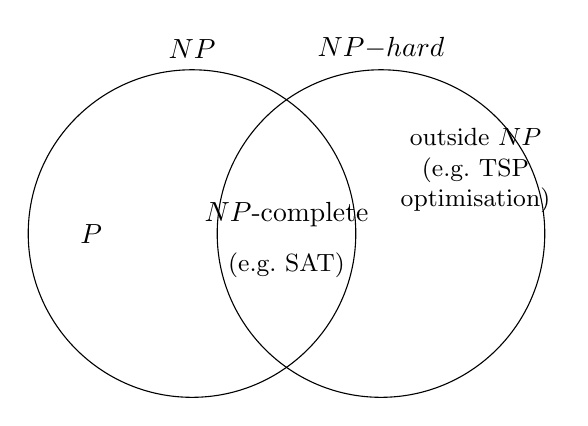
\begin{tikzpicture}[scale=0.8]
 \draw (0,0) circle (2.6cm) node[above,yshift=2.1cm] {$NP$};
 \draw (3,0) circle (2.6cm) node[above,yshift=2.1cm] {$NP\text{-hard}$};
 \node at (-1.6,0) {$P$};
 \node[align=center] at (1.5,0.3) {$NP$-complete};
 \node[align=center,font=\small] at (1.5,-0.5) {(e.g.\ SAT)};
 \node[align=center,font=\small] at (4.5,1.0) {outside $NP$\\(e.g.\ TSP\\optimisation)};
\end{tikzpicture}
\end{center}
\begin{center}
\small NP-complete $=$ NP $\cap$ NP-hard (drawn assuming $P\ne NP$)
\end{center}

\subsection{Sums and summation}
\label{sec:6-10}
% CN 6.10

\begin{definition}[Summation notation]
$\displaystyle\sum_{k=1}^n a_k = a_1+a_2+\cdots+a_n$. The variable $k$ is a dummy variable: renaming it does not change the sum.
\end{definition}

\begin{example}[Swapping the order of a double sum]
Consider $\sum_{i=1}^{n}\sum_{j=1}^{i} j$, the sum of the triangular array whose row $i$ is $1,2,\dots,i$:
\[
\begin{array}{c|ccccc}
i \backslash j & 1 & 2 & 3 & \cdots & n \\\hline
1 & 1 & & & & \\
2 & 1 & 2 & & & \\
3 & 1 & 2 & 3 & & \\
\vdots & \vdots & \vdots & & \ddots & \\
n & 1 & 2 & 3 & \cdots & n
\end{array}
\]
Summing row by row gives $1+(1+2)+(1+2+3)+\cdots+(1+\cdots+n)$. Summing column by column instead, column $j$ contains the value $j$ once for each row $i=j,\dots,n$, i.e.\ $n-j+1$ times. So
\[
\sum_{i=1}^{n}\sum_{j=1}^{i} j = \sum_{j=1}^{n}\sum_{i=j}^{n} j = \sum_{j=1}^n j(n-j+1).
\]
Both describe the same region $1\le j\le i\le n$, once ``by rows'' and once ``by columns''.
\end{example}

\subsection{Finite series}
\label{sec:6-11}
% CN 6.11

\begin{definition}[Series, partial sum]
A \emph{finite series} is the sum of the terms of a finite sequence. For an infinite sequence $(a_k)$, the $n$-th \emph{partial sum} is $S_n=\sum_{k=1}^n a_k$.
\end{definition}

\subsection{Finite arithmetic series}
\label{sec:6-12}
% CN 6.12

\begin{theorem}
\[
\sum_{k=1}^n \bigl(a+(k-1)d\bigr) = n\cdot\frac{2a+(n-1)d}{2} = n\cdot\frac{\text{first}+\text{last}}{2}.
\]
In particular, $1+2+\cdots+n=\dfrac{n(n+1)}{2}$.
\end{theorem}
\begin{proof}
Write the sum $S$ forwards and backwards and add term by term. Each of the $n$ pairs adds to $a+\bigl(a+(n-1)d\bigr)=2a+(n-1)d$, so $2S=n\bigl(2a+(n-1)d\bigr)$.
\end{proof}

\begin{example}
$1+3+5+\cdots+99$ has $50$ terms, so it equals $50\cdot\frac{1+99}{2}=2500=50^2$.
\end{example}

\subsection{Finite geometric series}
\label{sec:6-13}
% CN 6.13

\begin{theorem}
For $r\neq1$,
\[
\sum_{k=0}^n ar^k = a\cdot\frac{r^{n+1}-1}{r-1}.
\]
\end{theorem}
\begin{proof}
Let $S=a+ar+\cdots+ar^n$. Then $rS=ar+ar^2+\cdots+ar^{n+1}$, and subtracting, all but two terms cancel: $rS-S=ar^{n+1}-a$. Divide by $r-1\ne0$.
\end{proof}

\begin{example}
$1+2+4+\cdots+2^n=2^{n+1}-1$ (with $a=1$, $r=2$), as in Exercise 3.7.
\end{example}

\subsection{Infinite geometric series}
\label{sec:6-14}
% CN 6.14

\begin{theorem}[Convergence condition]
The infinite geometric series $\sum_{k=0}^\infty ar^k$ (with $a\ne0$) converges if and only if $|r|<1$, and then its sum is $\dfrac{a}{1-r}$.
\end{theorem}
\begin{proof}
The partial sums are $S_n = a\dfrac{1-r^{n+1}}{1-r}$. If $|r|<1$ then $r^{n+1}\to0$ (\S\ref{sec:6-8}), so $S_n \to \dfrac{a}{1-r}$. If $|r|\ge1$, the terms $ar^k$ do not tend to $0$, so the partial sums cannot settle down to a limit.
\end{proof}

\begin{example}
$\frac12+\frac14+\frac18+\cdots=\dfrac{1/2}{1-1/2}=1$, and $0.999\ldots=\dfrac{9/10}{1-1/10}=1$.
\end{example}

\subsection{Harmonic numbers}
\label{sec:6-15}
% CN 6.15

\begin{definition}[Harmonic numbers]
The $n$-th \emph{harmonic number} is $H_n = 1+\frac12+\frac13+\cdots+\frac1n$.
\end{definition}

\begin{theorem}[The harmonic series diverges]
$H_n\to\infty$ as $n\to\infty$, even though $1/n\to0$.
\end{theorem}
\begin{proof}
Group the terms of $H_{2^k}$ in blocks:
\[
H_{2^k} = 1 + \frac12 + \left(\frac13+\frac14\right) + \left(\frac15+\cdots+\frac18\right) + \cdots + \left(\frac{1}{2^{k-1}+1}+\cdots+\frac{1}{2^k}\right).
\]
The $j$-th block has $2^{j-1}$ terms, each at least $1/2^j$, so it adds up to at least $\frac12$. There are $k$ blocks after the first term, so $H_{2^k} \ge 1+\frac{k}{2}$. This tends to $\infty$, and $H_n$ is increasing, so $H_n\to\infty$.
\end{proof}

\begin{note}[Same bound, two proofs]
This is the bound $H_{2^n}\ge1+n/2$ proved by induction in \S\ref{sec:3-11}; here it comes directly from grouping.
\end{note}

\begin{note}[Growth rate]
$H_n$ grows like $\log_e n$: in fact $H_n - \log_e n \to \gamma = 0.5772\ldots$ (Euler's constant), so $H_n\approx\log_e n+\gamma$ for large $n$. It is unknown whether $\gamma$ is rational.
\end{note}

\begin{note}[A borderline case]
$(1/2^n)$ and $(1/n^2)$ tend to $0$ and have finite sums, but $(1/n)$ also tends to $0$ yet has an infinite sum: it decays just too slowly.
\end{note}
